\chapter{Beskrivelse}
Chain of responsibility (COR) er et software pattern, der mindsker koblingen mellem sender og reciever. Princippet er, at afsenderen/klienten kun kender en abstrakt 'handler'. Handleren har en kæde af nedarvede klasser, så handleren selv sørge for at håndtere et request ved at kalde rundt i kæden. 
Dette opnås ved, at der oprettes en abstrakt klasse 'Handleren'. Denne klasse indeholder en abstrakt-metode til at handle et request fra klienten.\\
Den abstrakte-metode bliver implementeret i de konkrete handlere, der er nedarvede fra den abstrakte handler klasse. I handler-metoden i de konkrete klasser bliver der checket på om requestet skulle handles af klassen. Hvis dette er tilfældet er bliver requestet handled og retuneret, dermed bliver kæden stoppet. Hvis requestet derimod ikke var til klassen, bliver requestet videresendt til den næste handler i kæden. Dette fortsætter indtil, at requestet er håndteret eller kæden slutter. \\

\noindent Klassediagrammet for strukturen af COR ses i figur \ref{fig:Klassediagram}.
\begin{figure}[H]
	\centering
	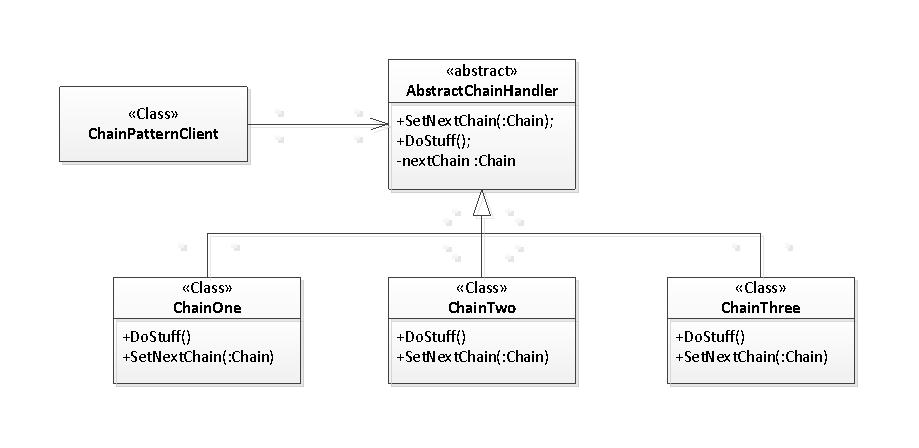
\includegraphics
	[width=140mm]{figures/UML.pdf}
	\caption{Klassediagram for Chain of Responsibility}
	\label{fig:Klassediagram}
\end{figure} 

\noindent Som det ses af klassediagramet indeholder den abstrakte klasse også metoden 'SetNextChain', der grunden til at klassen er abstrakt. Denne metode sætter, det næste led i kæden.

Kæden bliver i praksis defineret programmet. Hvilket gør at det kan være svært at overføre til andre sammenhængen uden at modificere koden.